In questo capitolo verrà mostrato il processo che porta alla compilazione del processo Go in un componente Wasm.\\

Se la fase di generazione è avvenuta con successo, all'interno del progetto dovrebbe essere presente una cartella chiamata \texttt{gen}, contenente diverse sotto-cartelle con il codice necessario per compilare i moduli Wasm.

\texttt{project/}
\dirtree{%
.1 workflow.yaml.
.1 tasks/.
.1 gen/.
.2 example\_component1.
.2 example\_component2.
}

\section{Wasm Builder}

A questo punto può essere invocato il componente \texttt{build}, che sostanzialmente esegue le seguenti operazioni:
\begin{enumerate}
    \item Istanzia il client Docker utilizzando l'apposito SDK\footnote{\url{https://pypi.org/project/docker/}}.
    \item Controlla se l'immagine \texttt{wash-build-image:latest} è presente. Se non lo è procede a buildarla utilizzando il dockerfile configurato.
    \item Per ogni cartella presente dentro \texttt{gen} istanzia un container con \texttt{wash-build-image} come immagine e monta la cartella all'interno del container.
    \item Attende la terminazione dei container.
\end{enumerate}

Si può notare come in questo caso le operazioni svolte dal framework siano limitate: la logica di build del componente e la pubblicazione dell'artifact OCI sono infatti delegate alle istanze in esecuzione su Docker.
    
\subsection{Wash build image}

Approfondiamo ora il meccanismo utilizzato per compilare i componenti Wasm, iniziando dal Dockerfile che descrive l'immagine di base utilizzata, mostrato nel Listing \ref{code:wash_buil_image_dockerfile}.

\begin{lstlisting}[language=Dockerfile, caption={wash-build-image Dockerfile}, captionpos=b, label={code:wash_buil_image_dockerfile}, basicstyle=\ttfamily\small]
FROM ubuntu:24.04 AS wash-build-image

# Install dependencies and tools
RUN apt-get update && apt-get install -y curl wget tar ...

# ----------------- Install WasmCloud -----------------
RUN curl -s "https://packagecloud.io/install/repositories/wasmcloud/core/script.deb.sh" | bash && \
    apt-get install -y wash

# ----------------- Install Go 1.23 -----------------    
RUN wget https://go.dev/dl/go1.23.4.linux-amd64.tar.gz && \
    tar -C /usr/local -xzf go1.23.4.linux-amd64.tar.gz && \
    rm go1.23.4.linux-amd64.tar.gz

# Set Go environment variables
ENV PATH="/usr/local/go/bin:${PATH}"
ENV GOPATH="/go"
ENV GOROOT="/usr/local/go"

# ----------------- Install TinyGo 0.34.0 -----------------
RUN wget https://github.com/tinygo-org/tinygo/releases/download/v0.34.0/tinygo_0.34.0_amd64.deb && \
    dpkg -i tinygo_0.34.0_amd64.deb && \
    rm tinygo_0.34.0_amd64.deb

# ----------------- Install Rust -----------------
# Install Rust
RUN curl https://sh.rustup.rs -sSf | sh -s -- -y && \
    . "$HOME/.cargo/env" && \
    cargo install --locked wasm-tools

# Set Rust environment variables
ENV PATH="/root/.cargo/bin:${PATH}"

# Verify installations
RUN go version && tinygo version && cargo --version && wash --version && wasm-tools --version

# ----------------- Build the WasmCloud module -----------------
FROM wash-build-image

RUN mkdir /app
WORKDIR /app

# Install go dependencies, build the wasm module, push it to the registry
CMD ["sh", "-c", "go env -w GOFLAGS=-buildvcs=false && go mod download && go mod verify && wash build && wash push $REGISTRY build/*.wasm && chown -R ${HOST_UID}:${HOST_GID} ."]
\end{lstlisting}

Il Dockerfile è strutturato in due fasi:
\begin{enumerate}
    \item \textbf{Fase 1}: vengono installate le dipendenze di Go, TinyGo, Rust e la shell di wasmCloud.
    \item \textbf{Fase 2}: viene predisposta l'immagine per la compilazione dei moduli Wasm.
\end{enumerate}

La preparazione della compilazione avviene dentro l'istruzione CMD, che infatti contiene:
\begin{itemize}
    \item Istruzioni per risolvere le dipendenze di go ed installarle nel progetto. In questo modo l'utente può aggiungere librerie supportate e il builder si occuperà di installarle nel progetto.
    \item Comando \texttt{wash build} che esegue la compilazione del progetto e genera il componente Wasm all'interno della cartella \texttt{gen}.
    \item Comando \texttt{wash push} che pubblica il componente Wasm come artifact OCI sul registry passato come configurazione.
    \item Istruzione per impostare i permessi sui file generati, necessario per poter gestire correttamente i files tramite Python.
\end{itemize}

\subsection{Istanziamento container}

Questo approccio consente di utilizzare una sola immagine per tutte le operazioni di build: le configurazioni dinamiche avvengono tramite variabili d'ambiente e i file da buildare vengono montati come volume al posto della cartella \texttt{/app}, come possiamo notare dal Listing \ref{code:build} contenente un estratto di codice del componente \texttt{build}:

\begin{lstlisting}[language=python, caption={Build componente Wasm con Docker}, captionpos=b, label={code:build}]
def __build_wasm(task_dir, client, reg_user, reg_pass, detached, wait_list):
    oci_url = wadm['spec']['components'][0]['properties']['image']
    name = wadm['spec']['components'][0]['name'] + '-build'
    ...
    # Build componente Wasm
    print(f" - Building WASM module {oci_url}")
    container = client.containers.run(
        "wash-build-image:latest",
        environment=[f'REGISTRY={oci_url}',
                     f'WASH_REG_USER={reg_user}',
                     f'WASH_REG_PASSWORD={reg_pass}',
                     f'HOST_UID={uid}',
                     f'HOST_GID={gid}'],
        volumes={os.path.abspath(task_dir): {'bind': '/app', 'mode': 'rw'}},
        remove = True,
        detach = True,
        name = name
    )
    
    # Build sequenziale o parallela
    if detached == 'False':
        container.wait()
    else:
        wait_list.append(name)
\end{lstlisting}

\subsection{Esecuzione parallelizzata}

Il processo di build può essere eseguito in modalità sequenziale o parallela, a seconda della configurazione delle variabili d'ambiente. Questo comportamento è gestito tramite la flag \texttt{detach}, che permette di avviare i container in modo asincrono. In questa modalità, viene utilizzata una waiting list per istanziare tutti i container in parallelo e attendere il completamento dell'operazione di build.\\

\section{Processo completo}

L'intero processo di build viene mostrato nella Figura [\ref{fig:impl_build}]:

\FloatBarrier
\begin{figure}[h]
    \centering
    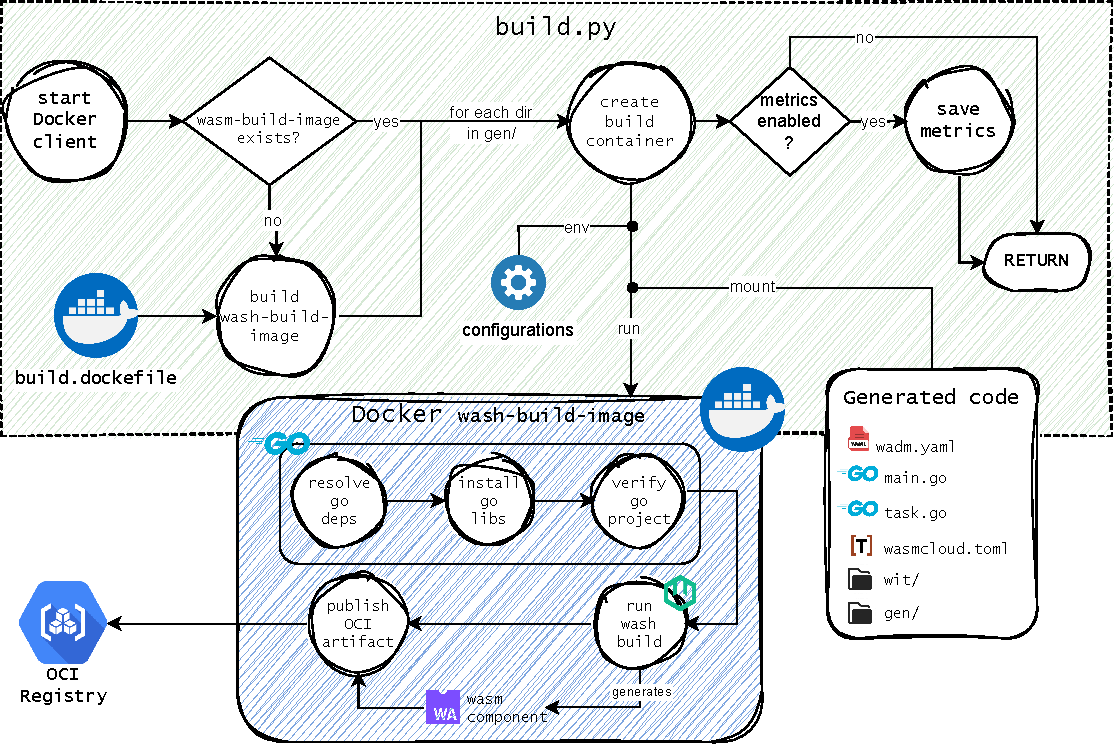
\includegraphics[width=\textwidth]{img/schemi/schemi-implementazione-build.drawio.pdf}
    \caption{Processo di Build componente Wasm}
    \label{fig:impl_build}
\end{figure}
\FloatBarrier